\documentclass{article}
\usepackage{graphicx}
\usepackage{bm}
\usepackage{amsmath}
\usepackage{amssymb}
\usepackage[toc,page]{appendix}
\usepackage{listings}
\usepackage{color}
\usepackage[margin=1.0in]{geometry}
\usepackage{fancyhdr}

\usepackage{etoolbox}
\patchcmd{\thebibliography}{\section*}{\section}{}{}

%\numberwithin{equation}{subsection}

\definecolor{mygreen}{rgb}{0,0.6,0}
\definecolor{mygray}{rgb}{0.5,0.5,0.5}
\definecolor{mymauve}{rgb}{0.58,0,0.82}

\lstset{ %
  backgroundcolor=\color{white},   % choose the background color; you must add \usepackage{color} or \usepackage{xcolor}
  basicstyle=\footnotesize,        % the size of the fonts that are used for the code
  breakatwhitespace=false,         % sets if automatic breaks should only happen at whitespace
  breaklines=true,                 % sets automatic line breaking
  captionpos=b,                    % sets the caption-position to bottom
  commentstyle=\color{mygreen},    % comment style
  deletekeywords={...},            % if you want to delete keywords from the given language
  escapeinside={\%*}{*)},          % if you want to add LaTeX within your code
  extendedchars=true,              % lets you use non-ASCII characters; for 8-bits encodings only, does not work with UTF-8
  frame=single,	                   % adds a frame around the code
  keepspaces=true,                 % keeps spaces in text, useful for keeping indentation of code (possibly needs columns=flexible)
  keywordstyle=\color{blue},       % keyword style
  language=Octave,                 % the language of the code
  otherkeywords={*,...},            % if you want to add more keywords to the set
  numbers=left,                    % where to put the line-numbers; possible values are (none, left, right)
  numbersep=5pt,                   % how far the line-numbers are from the code
  numberstyle=\tiny\color{mygray}, % the style that is used for the line-numbers
  rulecolor=\color{black},         % if not set, the frame-color may be changed on line-breaks within not-black text (e.g. comments (green here))
  showspaces=false,                % show spaces everywhere adding particular underscores; it overrides 'showstringspaces'
  showstringspaces=false,          % underline spaces within strings only
  showtabs=false,                  % show tabs within strings adding particular underscores
  stepnumber=2,                    % the step between two line-numbers. If it's 1, each line will be numbered
  stringstyle=\color{mymauve},     % string literal style
  tabsize=2,	                   % sets default tabsize to 2 spaces
  title=\lstname                   % show the filename of files included with \lstinputlisting; also try caption instead of title
}

\pagestyle{fancy}
\fancyhf{}
\rhead{Full Proposal}
\lhead{COMP SCI 6401 SP2016}
%\rfoot{Page \thepage}

\renewcommand{\thesection}{\Alph{section}}

\begin{document}

\title{Title}
\author{Edward Norris}

%\maketitle
%\thispagestyle{fancy}

%\begin{abstract}
%The abstract text goes here.
%\end{abstract}

%\tableofcontents

\section{Project Summary}\label{sec:A}
\subsection{Name and Degree Program}\label{sec:a1}
Edward Norris, PhD in Nuclear Engineering

\subsection{Project Title}\label{sec:a2}
An Evolutionary Algorithm for Online Spatial Discretization Optimization

\subsection{Project Description}\label{sec:a3}
Ionizing radiation is used extensively in many fields such as medicine, power production, and industrial non-invasive interrogation, however, utilization of such radiation poses a health concern to the surrounding populace. Engineering simulations are critical in determining the exposure to individuals in order to mitigate risks and ensure that proper protective measures are in place. However, these simulations are very time consuming, therefore, a two-phase scheme is used. First, the model is simulated with a relatively fast deterministic method utilizing a coarse spatial refinement mesh. This produces biasing parameters for the second phase, a high fidelity Monte Carlo calculation of exposure.

The success of the deterministic simulation in producing biasing parameters to accelerate the Monte Carlo code is highly dependent on the spatial discretization parameters selected. Unfortunately, selection of optimal parameters is very difficult and is typically tuned by experts. Experts well-versed in the nuances of developing good spatial discretizations are greatly outnumbered by those desiring such expertise; therefore, an evolutionary algorithm is proposed to perform the spatial discretization refinement. Evolutionary algorithms have shown promising results in similar engineering simulations for parameter tuning including other spatial discretization tuning.

The primary drawback of utilization of an evolutionary algorithm in practical application is that each fitness evaluation necessitates a fresh start of the Monte Carlo simulation, increasing runtime untenably. However, a unique property of the two-phase simulation scheme  is that the accelerating simulation does not impact the value of the final solution, only the convergence rate. Therefore, this work proposes to evolve discretization parameters online with respect to the Monte Carlo simulation. A single Monte Carlo simulation will continuously run and spatial discretizations will be swapped out during run-time. The statistical contribution from the current deterministic simulation can be calculated for the fitness function. Within the online framework, each discretization in the population can be evaluated until only its fitness is known to within some statistical threshold of other individuals. This allows pruning of poor solutions through early termination.


\subsection{Intellectual Merit}\label{sec:a4}
The current state-of-the-art in spatial discretization selection (specifically adaptive mesh refinement) utilizes octrees in 3D space. However, an octree mesh refinement is not applicable to the type of deterministic simulation used to accelerate the Monte Carlo code of interest. This necessitates development of a new representation of the spatial domain. Instead of a single octree population, three segment tree populations will be cooperatively co-evolved. Novel mutation and recombination operators will have to be constructed to operate on segment trees instead of octrees.

\subsection{Societal Benefit}\label{sec:a5}
Implementation of an evolutionary algorithm to automate generation of biasing parameters produced by a deterministic code for Monte Carlo acceleration will greatly enhance engineers' abilities to rapidly verify the safety of nuclear systems. Accurate simulations enable the dose to individual members of the public to be estimated so that systems can be optimized in order to reduce the health impact radiation imposes.

Further, benefits can be extended to any field that couples a non-stochastic simulation technique to generate biasing parameters for a Monte Carlo code. Such simulation systems are very prevalent in fluid dynamics, physics, heat transfer, and many other engineering fields.

\section{Project Narrative}\label{sec:b}
\subsection{Introduction}\label{sec:b1}
Monte Carlo simulations require detailed knowledge of the geometry of a system as well as type and location of radiation. With this information, a Monte Carlo simulation can calculate the dose to a person at a particular location due to the radioactive source(s). Radiation penetration through a shield is described as a Poisson process, meaning that the accuracy of a Monte Carlo simulation within some volume is inversely proportional to the square root of the number of particles in that volume. Therefore, in deep shielding problems, in which a strong source is attenuated (reduced in strength) greatly, the statistical uncertainty increases dramatically. 

In order to alleviate the high uncertainty in the analog Monte Carlo (so called due to it being directly analogous the physical transport process), biasing parameters are added to Monte Carlo simulations. Biasing parameters split important particles and kill unimportant ones to maximize the number of particles that reach the area of interest and reduce the computational overhead of tracking those that do not.

However, the production of accurate biasing parameters remains difficult. To remedy this, an adjoint transport calculation is made using a deterministic code. Rather than tracking particles forward through time as they traverse space and building a mesh of dose values, the adjoint solution tracks particles backward from an object of interest and builds a mesh of \textit{importance} to the region of interest.

Quantification of the effectiveness of a set of biasing parameters is done by calculating the figure of merit (FOM). The FOM is a metric used to compare the overall performance of two simulations and gives a directly comparable measure of performance for any two simulations as long as the physical problem being solved does not change and the computation hardware the two simulations were run on are identical. The FOM is defined in Eq.~\ref{eq:fom} where $T$ is the wall clock runtime of the simulation and $R$ is the estimated relative uncertainty of the output.
\begin{equation} \label{eq:fom}
FOM = \frac{1}{T R^2}
\end{equation}
Systems that use a deterministic solver to calculate the adjoint solution in order to produce biasing parameters for the primary Monte Carlo simulation are known as hybrid systems. One such system is AutomateD VAriaNce reducTion Generator (ADVANTG)~\cite{ref:Mosher2015} which is a framework developed at Oak Ridge National Laboratory specifically to produce biasing parameters for Monte Carlo N-Particle version~5 (MCNP)~\cite{ref:X5}, a Monte Carlo code developed by Los Alamos National Laboratory for radiation transport. 

However, currently available general-purpose radiation transport hybrid systems require a user defined spatial discretization in the form of a Cartesian grid~\cite{ref:Wagner2014, ref:Mosher2015}. This work will develop an evolutionary algorithm to optimize the spatial discretization grid for ADVANTG which will accelerate MCNP, these two codes have been coupled together very successfully~\cite{ref:Blakeman2007, ref:Risner2013, ref:Ibrahim2011, ref:Wagner2011}.

%The weight windows are used for particle rouletting and splitting. When a particle of weight $w_p$ moves into a region of weight $w_R$ that is higher than the particles weight, it may be split into multiple particles, each of the higher weight. Conversely, if the particle moves into a region of lower weight than itself, there is a chance it will be killed; surviving particles have their weight updated to the lower weight. Between these two biasing techniques, particles that have low probability of reaching a area of interest can be killed, reducing simulation time, and other particles can artificially be propogated through a highly attenuating medium.


\subsection{Related Work}\label{sec:b2}
In modern deterministic algorithms, spatial refinement is performed with a quadtree in 2D or an octree in 3D. However, quadtree/octree geometries cannot be utilized in the ADVANTG framework, instead, a structured Cartesian grid is required. A comparison of a 2D quadtree geometry and a 2D structured grid is shown in Fig.~\ref{fig:treecomp}. 

%Solutions have been shown to increase as the refinement increases, however, it has also been shown that, in increasing the discretization may only decrease the relative error by a marginal amount while increasing the computational time immensely [cite?]. Adaptive discretizations, for example, in the angular domain have little performance gain over their standard counterparts, except when large discontinuities are present in the problem~\cite{ref:jarrell2010}.
\begin{figure}
    \centering
    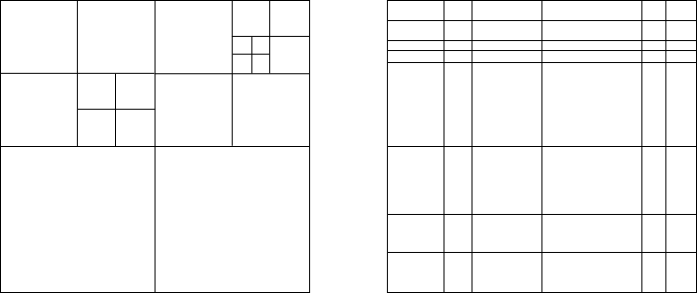
\includegraphics[width=3.0in]{treecomp}
    \caption{(Left) A 2D quadtree spatial representation. (Right) A structured Cartesian grid spatial representation.}
    \label{fig:treecomp}
\end{figure}

Octrees have been in use since 1980~\cite{ref:jackins1980249} to represent 3D space and have since been extended to K-trees to represent higher dimensional problems~\cite{ref:jackins1983533}. Octrees have been shown to be highly successful representing Cartesian geometry for computational engineering problems, particularly for adaptive mesh refinement~\cite{ref:Linden201558}. Oct-trees have also been used successfully to decompose image space, including 2D images~\cite{ref:Lange2004592} and 3D images~\cite{ref:udomchaiporn2013229, ref:Lee2010359}. Octrees have even been used directly in Monte Carlo simulations for radiative transfer of dust~\cite{ref:Saftly2013} that track voxels rather than individual particles.

Octree structures remain inefficient in particle tracking Monte Carlo simulations due to the additional computational overhead. At every step in the path of every particle, its intersection with all bounding surfaces of the voxel containing it must be calculated. Such calculations are extremely fast in structured Cartesian grids, but much slower in unstructured meshes. Therefore, MCNP only supports structured Cartesian grids as input for biasing parameters.

Though the physical representation of space is different between octree methodology and the proposed segment-tree methodology, both share a similar tree-like structure that represents a physical space. Therefore, a survey of evolutionary algorithms that evolve octrees and similarly structured trees could prove beneficial in the development of evolutionary operators.

Many evolutionary algorithms have been used in the past that involve octrees but do not directly evolve them. They are often used as a medium to partition some space into a structure more suited for evolutionary computing ~\cite{ref:Zhu2015301, ref:Schwertfeger200853}. While these applications do not directly evolve the spatial discretization itself, some insight into applicable operators can still be gleaned from them. For example, Laszlo and Mukherjee developed an algorithm to assist in $k$-means clustering by building a quadtree and using selected nodes as an initial guess for the $k$-means clustering algorithm~\cite{ref:Laszlo2006}. Though the octree itself was not evolved, Laszlo and Mukherjee highlighted that the refinement density in space can be leveraged to produce more effective crossover operators.

Majeed and Ryan proposed special version of the one point crossover operator for GP that takes advantage of the structure of the parent trees to produce more optimized offspring~\cite{ref:Majeed2007}. Seo and Goodman extended this work by adding a similar mutation operator that maintains a structural metric in order to explore the search space in a more complete fashion~\cite{ref:seo2009}.

In evolutionary algorithms, the fitness function can be noisy~\cite{ref:Jin2005}.

In \cite{ref:Liapis2015} a constrained novelty search is performed.

In \cite{ref:smith2015} it is shown that novelty alone is often insufficient.

Often they evolve Pareto fronts~\cite{ref:Bucci2005}. However, in long eval time fitness functions of more than two populations this becomes infeasible.

must avoid relative overgeneralization which finds \textit{robust} solutions over optimal solutions.

Therefore, novelty selection is proposed. This is similar to~\cite{ref:Lehman2011}.

\textbf{Add segment trees and co-evolution}

\subsection{Proposed Research}\label{sec:b3}
Some words should go here maybe?

\subsubsection{Representation}
Each of the $x$, $y$, and $z$ axes will be represented as a segment tree. In a segment tree, a single dimension of space is recursively divided into sub-segment trees until the leaf nodes are reached. The leaf nodes consist of discrete points along that dimension. An example segment tree along an axis from 0 to 1 is shown in Fig.~\ref{fig:segtree}.

% Crossover
\subsubsection{Crossover}
Since neighbors in the segment tree are also neighbors in physical space, it is expected that unique evolutionary operators can be devised to leverage these aspects. In the proposed segment tree, there is a unique constraint in that every leaf node must be strictly greater than the node to its left and strictly less than the node to its right. Standard crossover operators cannot be applied since they will almost similarly violate this monotonicity constraint. There are a number of ways to alleviate this, first, the standard crossover could be applied and then a repair algorithm is applied which rearranges the tree into a valid structure. Alternatively, branches from one tree could be selectively chosen to replace specific other branches, though some kind of repair function would again be necessary. Both of these options will be implemented and compared.

% Mutation
\subsubsection{Mutation}
Two kinds of mutation are considered in this work, the first operates on all segments on the tree, the second only on a subset of leaf nodes. The first mutation operator will shift all points either to the left or right by some amount, this will allow regions of high point density to travel and explore the search space. The second mutation operator will \textit{only} be applied to nodes in the segment tree that are direct parents of leaf nodes. They will either have more leaf nodes added, increasing point density, or have them pruned, reducing their density. The combination of these two mutation operators is expected to allow regions of high density to travel while simultaneously allowing new exploration.

% Fitness eval
\subsubsection{Fitness Evaluation}
While swapping out the biasing parameters of MCNP during runtime would be advantageous in some respects, it would complicate the comparison of the fitness of individuals. Therefore, an artificial online algorithm is proposed. Two separate runs of $N_1$ and $N_2$ particles produce dose values $D_1$ and $D_2$ with uncertainty $R_1$ and $R_2$ respectively. The combined dose, $D$, and uncertainty, $R$, can be computed with Eq.~\ref{eq:mean_combine} and ~\ref{eq:stddev_combine} respectively~\cite{ref:knoll2000}. Utilizing Eq.~\ref{eq:mean_combine} and~\ref{eq:stddev_combine}, results of any number of MCNP runs can be combined to produce a result statistically indistinguishable from a true online solution.
\begin{equation}\label{eq:mean_combine}
D = \frac{N_1}{N_1 + N_2} D_1 + \frac{N_2}{N_1 + N_2} D_2 \\
\end{equation}
\begin{equation}\label{eq:stddev_combine}
R = \sqrt{\left( \frac{N_1}{N_1 + N_2}\right)^2 R_1 + \left( \frac{N_2}{N_1 + N_2}\right)^2 R_2}
\end{equation}

The evolutionary algorithm will be run on a series of toy problems created only to demonstrate its effectiveness as well as benchmark problems given in~\cite{ref:Mosher2015}. The benchmark results will be compared to results obtained from expert generated biasing parameters.

\begin{figure}
    \centering
    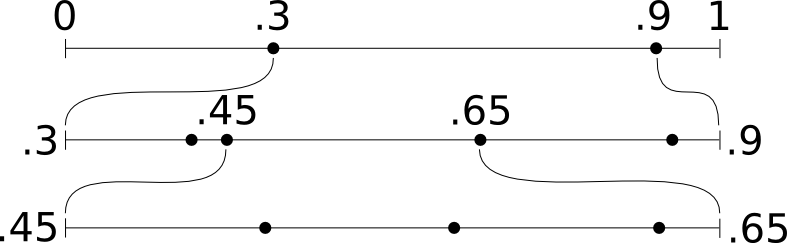
\includegraphics[width=3.0in]{treeex}
    \caption{Segment tree example for a single axis.}
    \label{fig:segtree}
\end{figure}

%Co-Evolution
\subsubsection{Co-Evolution}
Three populations of segment trees will be cooperatively co-evolved. What necessiates this? 

One of the key challenges will be pairing individuals in a meaningful manner. Since there are three populations, random 20 way selection is difficult. However, the selections could be made at random for each pool.

% Termination
\subsubsection{Termination}
The evolution is guaranteed to be stopped prematurely. The global figure of merit is defined by

\begin{equation}
FOM_{global} = \frac{1}{\sum \left( T_{ADV} + T_{MC} \right) R^2}
\end{equation}

\begin{equation}\label{eq:stddev_combine}
R = \sqrt{\sum_i \left( \frac{N_i}{N_{TOTAL}} \right)^2 R_i}
\end{equation}

The evolution stops when the expected probability that further improvment in the population will no longer more than pay for the time cost of executing the EA drops below 50\%. Of course, this probability can only be estimated based on historical data the previous generations.

\subsection{Qualifications and Resources}\label{sec:b4}
The PI is a PhD student in nuclear engineering with over five years of experience with MCNP and whose research work involves usage of both MCNP and ADVANTG on a daily basis. The PI is concurrently pursuing a MS in computer science and has working knowledge of EAs from previous coursework.

The PI has access to an i7-5960x desktop computer representative of the target platform for this algorithm. While running the optimization algorithm on a cluster or similar high performance system would be preferable, there are stringent export control issues that prevent running MCNP on general computing clusters. 

\subsection{Tentative Work Plan}\label{sec:b5}
During the remaining ten weeks before the final deadline, the tentative work plan is as follows:

\begin{description}
\item[Week 1] Develop and implement a simple hill climber that will conclusively show that the solution space is not convex and that the three dimensions cannot be evolved independently, to justify the co-evolutionary component of the proposal.

\item[Week 2-3] Write the full proposal and develop the framework that will evolve the spatial discretization including the post-processing necessary to read the MCNP output format.

\item [Week 4-6] Develop and test evolutionary operators.

\item [Week 7] Tune evolutionary parameters (population size, mutation rate, etc.).

\item [Week 8] Run evolutionary algorithm on simple benchmark cases.

\item [Week 9] Write final report.

\item [Week 10] Contingency week.
\end{description}

The greatest risk in this endeavor is that the EA will fail to converge within an acceptable timeframe. In this event, the evolutionary operators will have to be modified to incorporate more problem specific information, though this would be detrimental to the overall generality of the proposed solution. Further, a user supplied initial population to assist in early evolution, when many individuals are of sufficiently low quality that comparing them is difficult due to statistical noise, may be necessary.

\section{New Work}
There has been stuff done.

In the XYZ order, the optimum was 30x5x50 with a fitness of 520.5. It took 1612.8 seconds to compute this result.

\begin{figure}
    \centering
    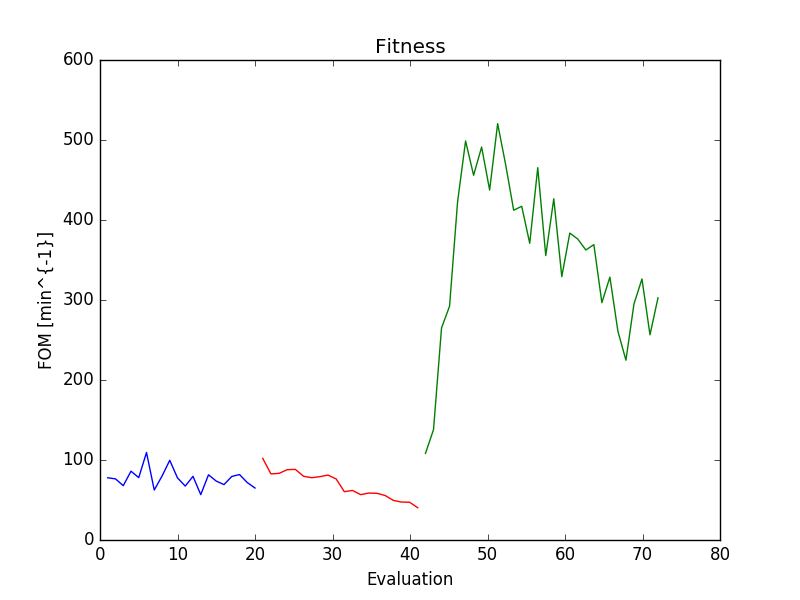
\includegraphics[width=3.0in]{fitness_xyz}
    \caption{XYZ Fitness}
    \label{fig:fitness_xyz}
\end{figure}

\begin{table}
\begin{center}
\label{tbl_decay}
\caption{The work done so far for Analog using 10 threads}
\begin{tabular}{|c|c|c|c|c|c|c|}
\hline
\textbf{Histories} & \textbf{Time [min]} & \textbf{Escape} & \textbf{Counts} & \textbf{Flux} & \textbf{Unc} & \textbf{FOM} \\ \hline
$10^4$ & .01 & 1 & 0 & 0 & -- & -- \\ \hline
$10^5$ & .01 & 2 & 0 & 0 & -- & -- \\ \hline
$10^6$ & .04 & 28 & 0 & 0 & -- & -- \\ \hline
$10^7$ & .31 & 345 & 2 & 6.08633E-9 & .9381 & 3.67 \\ \hline
$10^8$ & 3.03 & 3066 & 11 & 3.23058E-9 & .3477 & 2.73 \\ \hline
$10^9$ & 30.07 & 31247 & 167 & 4.40395E-9 & .0924 & 3.89 \\ \hline
\end{tabular}
\end{center}
\end{table}

\begin{table}
\begin{center}
\label{tbl_decay2}
\caption{The hillclimber $x \rightarrow y \rightarrow z$ using 10 threads}
\begin{tabular}{|c|c|c|c|c|c|c|c|}
\hline
$N_x$ & $N_y$ & $N_z$ & $T_{ADV}$ & $T_{MC}$ & \textbf{Flux} & $R$ & $FOM$ \\ \hline
10 &  5 &  5 & .033 & .434 & 5.03892E-9  & 0.0918 & 254 \\ \hline
15 &  5 &  5 & .033 & .406 & 4.63118E-9  & 0.0813 & 345 \\ \hline
20 &  5 &  5 & .038 & .391 & 5.37490E-9  & 0.0776 & 392 \\ \hline
25 &  5 &  5 & .044 & .364 & 4.76957E-9  & 0.0727 & 464 \\ \hline
30 &  5 &  5 & .036 & .351 & 4.14858E-9  & 0.0731 & 486 \\ \hline
40 &  5 &  5 & .043 & .342 & 4.40428E-9  & 0.0780 & 427 \\ \hline
50 &  5 &  5 & .044 & .318 & 4.50058E-9  & 0.0847 & 385 \\ \hline \hline

30 &  5 & 5 & .036 & .351 & 4.14858E-9  & 0.0731 & 486 \\ \hline
30 & 10 & 5 & .049 & .338 & 4.79677E-9  & 0.1041 & 238 \\ \hline
30 & 15 & 5 & .046 & .328 & 3.96065E-9  & 0.0774 & 446 \\ \hline
30 & 20 & 5 & .045 & .325 & 4.43592E-9  & 0.0835 & 388 \\ \hline
30 & 25 & 5 & .049 & .311 & 4.67980E-9  & 0.0895 & 347 \\ \hline \hline

30 &  5 &  5 & .036 & .351 & 4.14858E-9  & 0.0731 & 486 \\ \hline
30 &  5 & 10 & .044 & .541 & 4.47556E-09  & 0.0149 & 7700 \\ \hline
30 &  5 & 15 & .051 & 1.085 & 4.55868E-09  & 0.0060 & 24500 \\ \hline
30 &  5 & 20 & .054 & 2.062 & 4.56427E-09  & 0.0044 & 24300 \\ \hline
30 &  5 & 25 & .062 & 2.586 & 4.54842E-09  & 0.0030 & 42000 \\ \hline
30 &  5 & 30 & .073 & 3.359 & 4.55361E-09  & 0.0024 & 50600 \\ \hline
30 &  5 & 35 & .071 & 3.553 & 4.55024E-09  & 0.0022 & 57000 \\ \hline
30 &  5 & 40 & .073 & 4.033 & 4.54731E-09  & 0.0023 & 46000 \\ \hline \hline

10 & 10 & 10 & .083 & .801 & 4.54734E-9  & 0.0114 & 9610 \\ \hline
20 & 20 & 30 & .087 & 3.180 & 4.56038E-09  & 0.0024 & 53100 \\ \hline
30 & 30 & 40 & .199 & 3.678 & 4.55865E-09  & 0.0023 & 0 \\ \hline
30 & 30 & 35 & .185 & 2.897 & 4.55476E-09  & 0.0024 & 56300 \\ \hline
20 & 20 & 35 & .099 & 3.214 & 4.55958E-09  & 0.0023 & 56300 \\ \hline
10 & 10 & 35 & .059 & 3.936 & 4.54775E-09  & 0.0021 & 56800 \\ \hline
\end{tabular}
\end{center}
\end{table}



\bibliography{prop}{}
\bibliographystyle{acm}


\end{document}